% Required packages in the main preamble:
% \usepackage{graphicx}
% \usepackage{booktabs}
% \usepackage{tabularx}
% \usepackage{array}

\providecommand{\SysName}{CARE}

\section{Preliminaries}
\label{sec:preliminaries}

\SysName{} targets automated refactoring of C/C++ systems code, where even a small
source-level cleanup can silently change error propagation, resource ownership,
or security validation. This section defines the terminology and safety model
used throughout the paper.

\subsection{Security-Sensitive Refactoring}
\label{sec:prelim-refactoring}

Let $P$ denote a C/C++ program and let $\Delta$ denote a source-level patch.
Applying the patch yields a new program $P' = P + \Delta$. A refactoring is
intended to improve structure, reduce duplication, or make code easier to
maintain without changing the program's intended behavior. In systems code,
however, intended behavior includes more than ordinary return values: it also
includes error codes, cleanup ordering, ownership transfer, lock state, logging,
I/O, and validation checks that enforce security boundaries.

We call a refactoring \emph{behavior-preserving} if, for the executions in
scope, $P'$ preserves the externally visible behavior of $P$: return values,
observable side effects, API contracts, and error-handling conventions. We call
it \emph{security-preserving} if it does not weaken input validation, bounds
checks, null checks, resource lifecycle handling, or error cleanup behavior.
\SysName{} treats these properties conservatively: a patch is accepted only after it
passes the validation gates shown in Figure~\ref{fig:prelim-safety-model}.

\begin{figure}[t]
  \centering
  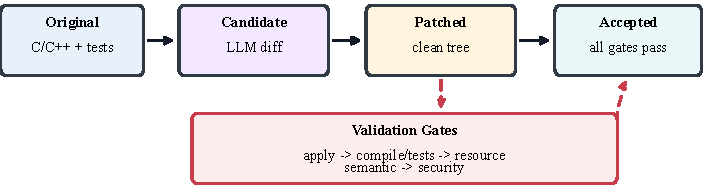
\includegraphics[width=\columnwidth]{img/care_prelim_safety_model.pdf}
  \caption{\SysName{}'s conservative safety model. An LLM-generated patch is first
  applied to a clean temporary project tree. \SysName{} accepts it only if the patch
  applies and passes syntactic, build/test, resource, semantic, and security
  regression checks. Passing these gates provides conservative evidence of
  safety; it is not a formal proof of full semantic equivalence.}
  \label{fig:prelim-safety-model}
\end{figure}

\subsection{Program Context}
\label{sec:prelim-context}

\SysName{} analyzes a project as a collection of source files, functions, control-flow
fragments, data-flow facts, and resource events. Table~\ref{tab:prelim-terms}
summarizes the core terms used in the rest of the paper.

\begin{table}[t]
  \centering
  \caption{Core \SysName{} terminology.}
  \label{tab:prelim-terms}
  \footnotesize
  \begin{tabularx}{\columnwidth}{@{}>{\raggedright\arraybackslash}p{0.30\columnwidth}>{\raggedright\arraybackslash}X@{}}
    \toprule
    \textbf{Term} & \textbf{Meaning in \SysName{}} \\
    \midrule
    Code location &
    File, line, and optional column used to anchor evidence, prompts, patches, and validation logs. \\
    Function summary &
    Function name, signature, body, and line range used as local LLM and detector context. \\
    Basic block &
    Lightweight statement group used to model branches, returns, gotos, and cleanup paths. \\
    Context edge &
    Typed relation such as call, control, data, goto, return, or resource-state edge. \\
    Resource event &
    Acquire/release action such as \texttt{malloc}/\texttt{free}, \texttt{fopen}/\texttt{fclose}, or lock/unlock. \\
    Context graph &
    Unified graph of functions, blocks, edges, resources, error paths, and side-effect summaries. \\
    Opportunity &
    Ranked candidate location with kind, severity, evidence, and a concise context summary. \\
    Patch candidate &
    LLM-generated unified diff accepted only after \SysName{} validation passes. \\
    \bottomrule
  \end{tabularx}
\end{table}

The central abstraction is the \emph{security-aware contextual refactoring graph}.
It can be viewed as a directed, typed graph
$G_c=(V,E,A)$, where $V$ contains function and basic-block nodes, $E$ contains
typed edges, and $A$ contains attributes such as source locations, resource
variables, side-effect summaries, and return-condition summaries. \SysName{} does not
require a complete formal model of the entire program. Instead, it constructs
enough local and interprocedural context to constrain patch generation and to
detect likely safety regressions.

\subsection{Refactoring Opportunities}
\label{sec:prelim-opportunities}

A refactoring opportunity is a detector-produced record
$o=(k,\ell,s,e,c)$, where $k$ is the opportunity kind, $\ell$ is the source
location, $s$ is the severity, $e$ is structured evidence, and $c$ is a concise
context summary. \SysName{} currently focuses on security-relevant refactorings common
in C/C++ code: duplicated cleanup logic, resource lifecycle imbalance, repeated
validation checks, dead or unreachable code, and general security smells.

\begin{table}[t]
  \centering
  \caption{\SysName{} opportunity classes.}
  \label{tab:opportunity-classes}
  \footnotesize
  \begin{tabularx}{\columnwidth}{@{}>{\raggedright\arraybackslash}p{0.33\columnwidth}>{\raggedright\arraybackslash}X@{}}
    \toprule
    \textbf{Class} & \textbf{Evidence and main safety risk} \\
    \midrule
    Goto-based redundancy &
    Repeated cleanup or chained labels. Risk: changing cleanup order, return code, or error-path side effects. \\
    Resource imbalance &
    Missing/double release or early return after acquire. Risk: leaks, double frees, double unlocks, or ownership confusion. \\
    Duplicate check &
    Repeated null, bounds, length, or status check. Risk: deleting a check that is not actually redundant. \\
    Dead or unreachable code &
    Code after unconditional return/goto or constant branch. Risk: deleting reachable cleanup or diagnostics. \\
    Security smell &
    Unsafe API, unchecked return, or inconsistent error propagation. Risk: masking a bug or changing error behavior. \\
    \bottomrule
  \end{tabularx}
\end{table}

Each detector emits both a severity label and structured evidence. \SysName{} uses
this evidence to decide whether an opportunity is suitable for LLM-based
refactoring. For example, a duplicate-check opportunity is considered safe only
when \SysName{} observes no assignment, mutating call, or obvious aliasing risk between
the two checks. Similarly, a resource opportunity must identify the relevant
resource variable and the acquire/release events involved.

\subsection{LLM Patch Candidates and Plans}
\label{sec:prelim-patches}

\SysName{} separates \emph{planning} from \emph{patch generation}. A refactoring plan
summarizes the patch intent, affected files and functions, required invariants,
security constraints, behavior-preservation goals, patch strategy, and validation
strategy. The plan is machine-readable and is used to constrain the LLM patch
generator.

A patch candidate is a unified diff paired with an explanation and confidence
score. \SysName{} treats LLM output as untrusted: a candidate may be syntactically
invalid, may edit the wrong file path, may fail to compile, or may introduce an
unsafe regression. Therefore, a candidate is not considered a \SysName{} result until
it survives validation. When validation fails, \SysName{} records the failure taxonomy
and may feed the logs back to the repair loop to request a smaller, safer patch.

\subsection{Validation Model}
\label{sec:prelim-validation}

The validator checks each candidate on a clean project state. First, \SysName{} repairs
common diff path mistakes and attempts to apply the patch. It then runs available
build and test commands, invokes optional static analyzers when installed, and
performs lightweight static checks for resource consistency, semantic
preservation, and security regressions. A validation result contains per-stage
outcomes, logs, and counterexamples. \SysName{} accepts a patch only if all required
stages pass.

The validation model is intentionally conservative. \SysName{} does not claim to prove
full semantic equivalence for arbitrary C/C++ programs. Instead, it aims to
reject patches that exhibit common unsafe symptoms: removed bounds or null
checks, changed public signatures, changed return forms, missing cleanup on error
paths, double releases, unchecked new allocations, or replacement of safer APIs
with unsafe ones. This conservative model is central to the paper's evaluation:
we report not only how often patches apply, but also how often they pass the
resource, semantic, and security gates.

\subsection{Scope and Assumptions}
\label{sec:prelim-scope}

\SysName{} is a research prototype, not a verified compiler transformation. The
current implementation assumes access to a source tree and, when available,
project-specific build and test commands. It can use compile databases and
clang-based confirmation when available, but it also includes lightweight
fallback analysis to support large-scale scans. The strongest claims in this
paper concern security-relevant C/C++ refactoring opportunities whose safety can
be checked using the contextual evidence and validation gates above. More complex
semantic changes, deep aliasing, concurrency protocols, and cross-component API
migrations are outside the current scope.
